Granular material is a family of material characterized by its large bulk of densely packed particles, ranging from nanometers to centimeters~\cite{introGranular2}, and is able to resist deformation and form heaps, i.e., behave like a solid and withstand strong shear force~\cite{introGranular3}. Simple examples of granular materials include sand, gravel, clays, seeds, nuts, and all ranges of powders such as coffee powder, cement powder, which is shown in figure~\ref{fig:granularExample}. Furthermore, many processes and equipments in chemical plants use granular materials, such as catalysis, adsorption, and heat exchangers. Granular materials are projected to make about half of the products and three-quarters of the raw materials used in the chemical industry~\cite{introGranular}. Thus, understanding how granular materials behave is of great significance. 

\begin{figure}[H]
    \centering
    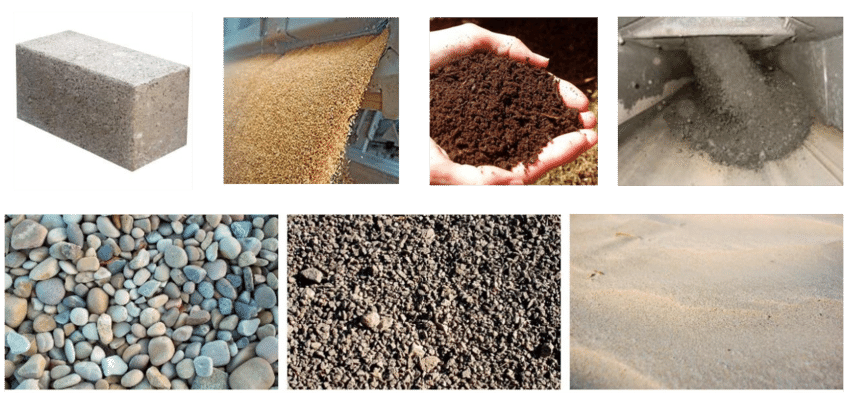
\includegraphics[scale=0.5]{granularExample.png}
    \caption{Examples of Granular Materials~\cite{granularExample}.}
    \label{fig:granularExample}
\end{figure}

The simulation of granular material's bulk mechanical behavior is done using Discrete Particle Model (DPM, or Discrete Element Method~-~DEM), which generates the movement of individual particles to capture the macro-scale behavior. The DPM is a family of numerical methods for computing the motion of a large number of particles~\cite{Weng:2015}, first proposed by Cundall and Strack in the 1970s~\cite{cundallstrack}.
Since the properties of granular materials differ wildly, these simulations require an extensive calibration process designed individually for each type of granular material. Some parameters of the granular material model can be measured directly, such as size distribution or density. However, other parameters are effective parameters (i.e., they result from a simplified particle model) and thus cannot be directly measured. These parameters are then calibrated by choosing a few standard calibration setups (rotating drum, heap test, ring shear cell) and simulating these setups in a DPM simulation, and the missing parameters are determined such that the response of the experimental and simulation setups match.

Recently, coupled with the raise of Machine Learning in other fileds, it has also been applied to solve the calibration problem. This has been done using a Neural Network~\cite{nn-calibration, NN-GA, NN-coarse, YE2019292}, Genetic Algorithm~\cite{ga-calibration}, and a recursive Bayesian sequential Monte-Carlo filtering algorithm named GrainLearning~\cite{grainLearning}. In this Assignment, three Machine Learning algorithms will be discussed: Neural Network, Random Forest (supervised model), and GrainLearning (unsupervised model). These three algorithms set to treat the calibration problem in two different ways: While GrainLearning looks to identify the microparameters from the experimental and DEM simulations's bulk parameters (inverse problem), the supervised models will help generating a database that can map different microparameters combinations to their corresponding bulk parameters, generated by DEM simulations. In other word, NN and RF will learn the built-in relationship between the micro- and macroparameters of the Discrete Particle Model, thus allow a much faster prediction compare to a full DEM simulation. One advantage of GrainLearning compares to other Machine Learning algorithms such as Neural Network is that it is an unsupervised learning algorithm, i.e., it can starts calibrating with a minimal amount of input information. However, each material needs calibration for multiple bulk parameters, i.e., Static Angle of Repose, Dynamic Angle of Repose, shear tester, etc.~since a set of microparameters that is valid for one bulk parameter might not valid for another~\cite{reviewCalibration}. Therefore, scaling up with a Neural Network model might be more simple, since a Neural Network can produces multiple valid combinations for each bulk parameter.  

In the next section, the characterisation and experimental method will be discussed, including static Angle of Repose, Discrete Particle Model, contact laws, and the material used in the simulation. Section~\ref{section:Calibration} will discuss in detail different approach and method of each model. The result of GrainLearning will be discuss in section~\ref{section:GLPerformance}, while section~\ref{section:supervisedPerformance} discuss the supervised model's performance. Subsequently, section~\ref{section:discussion} will compare the models, discuss the strength and weakness of each model, and the limitations.  ss
